\documentclass[tikz,border=8pt]{standalone}
\usepackage[T1]{fontenc}
\usepackage{lmodern}
\usetikzlibrary{arrows.meta,positioning,shapes.geometric,fit}
\definecolor{vmcblue}{HTML}{DCEEFF}
\definecolor{bunrakuorange}{HTML}{FFE4C4}
\definecolor{networkviolet}{HTML}{E9DDF7}
\definecolor{godotgreen}{HTML}{DDF3DF}
\definecolor{scyellow}{HTML}{FFF3BF}
\tikzset{
  box/.style={draw,rounded corners=3pt,very thick,align=center,minimum height=11mm,text width=34mm,font=\sffamily\small},
  smallbox/.style={box,text width=31mm},
  flow/.style={-{Latex[length=3mm]},very thick},
  net/.style={<->,>=Latex,very thick,dashed},
  networkflow/.style={-{Latex[length=3mm]},very thick,red},
  networknet/.style={<->,>=Latex,very thick,dashed,red},
  label/.style={font=\sffamily\scriptsize,align=center,fill=white,inner sep=1.5pt}
}
\begin{document}
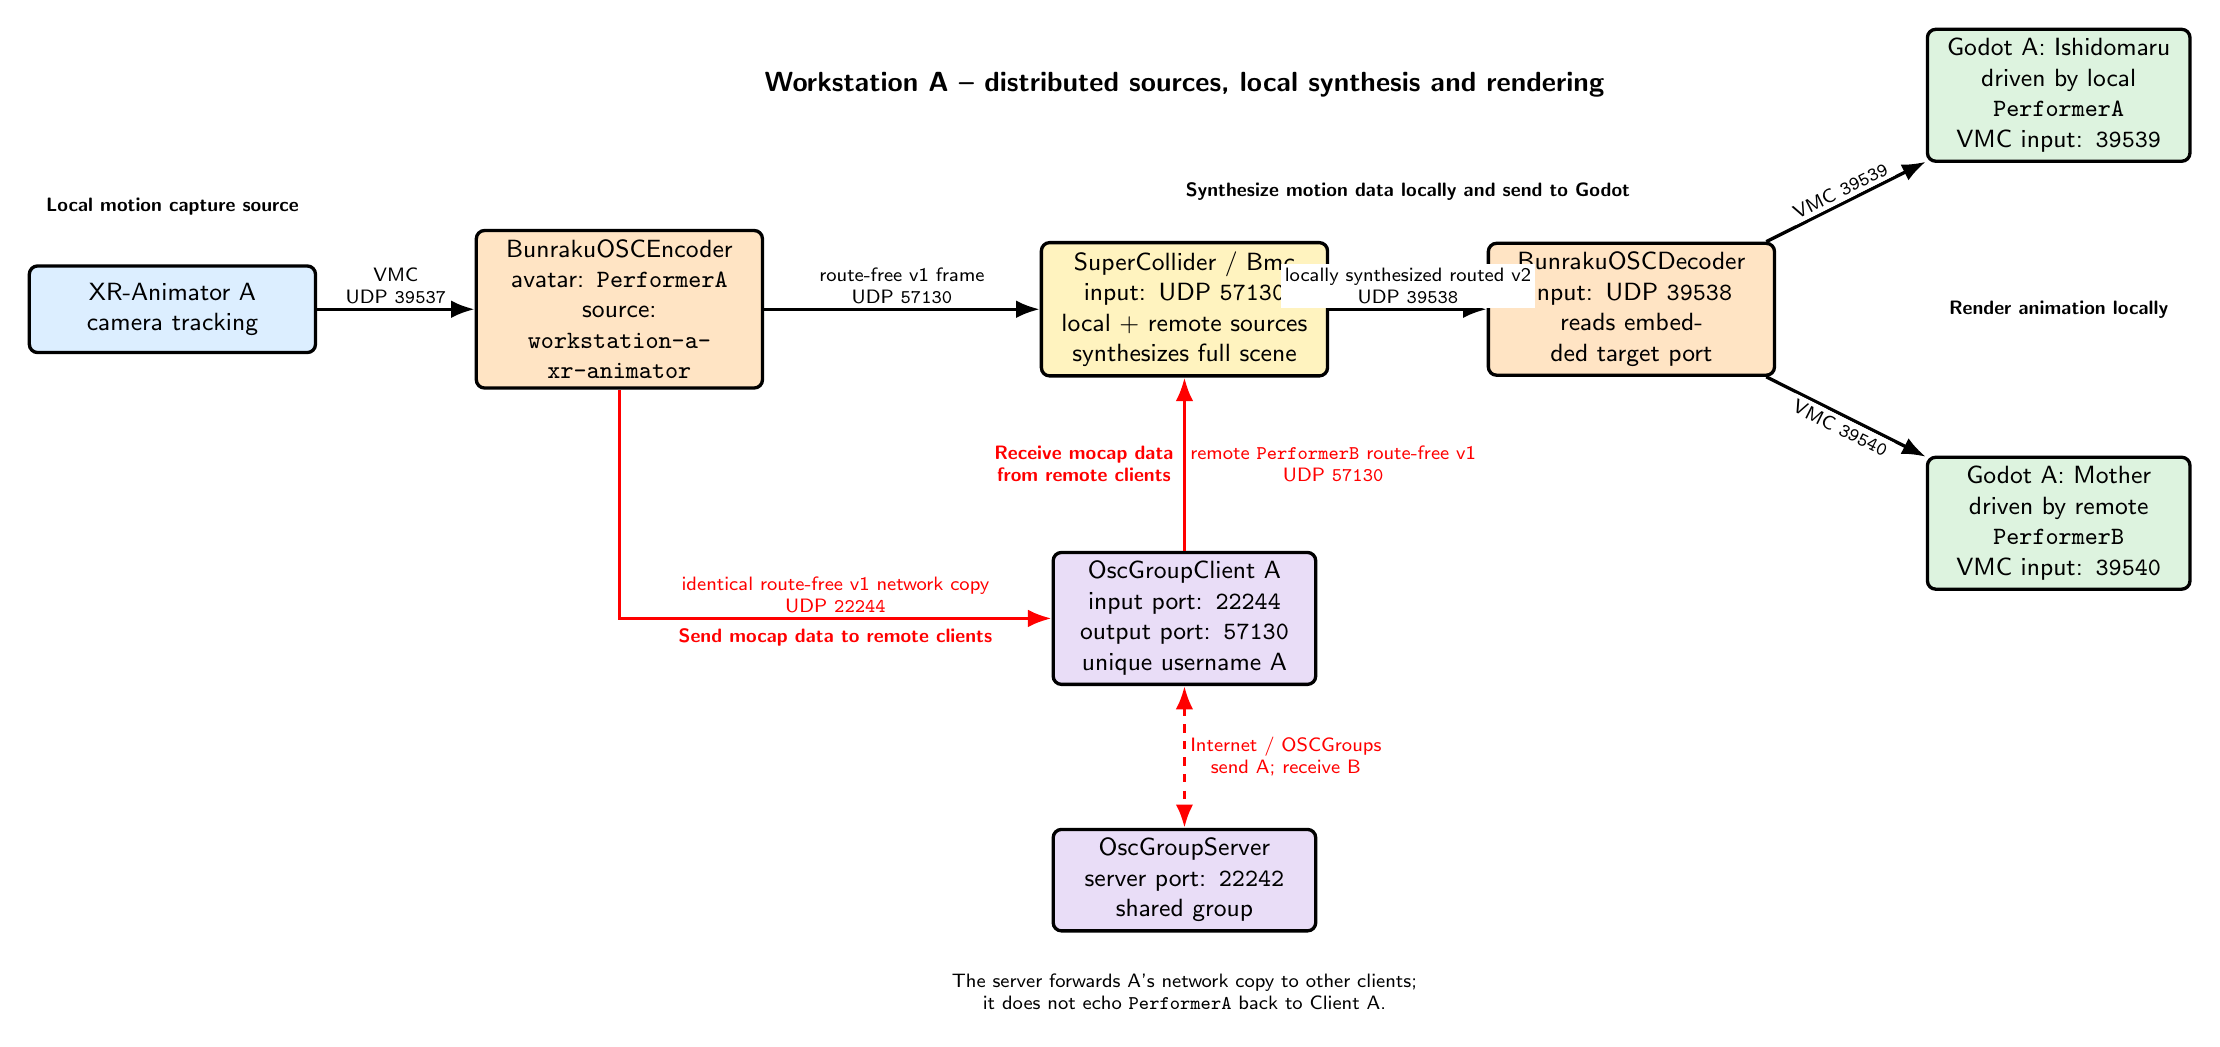
\begin{tikzpicture}[node distance=16mm and 20mm]
  \node[box,fill=vmcblue] (xr) {XR-Animator A\\camera tracking};
  \node[box,fill=bunrakuorange,right=of xr] (enc) {BunrakuOSCEncoder\\avatar: \texttt{PerformerA}\\source: \texttt{workstation-a-}\\\texttt{xr-animator}};
  \node[box,fill=scyellow,right=35mm of enc] (bmc) {SuperCollider / Bmc\\input: UDP \texttt{57130}\\local + remote sources\\synthesizes full scene};
  \node[box,fill=bunrakuorange,right=of bmc] (dec) {BunrakuOSCDecoder\\input: UDP \texttt{39538}\\reads embedded target port};

  \node[smallbox,fill=networkviolet,below=22mm of bmc] (client) {OscGroupClient A\\input port: \texttt{22244}\\output port: \texttt{57130}\\unique username A};
  \node[smallbox,fill=networkviolet,below=18mm of client] (server) {OscGroupServer\\server port: \texttt{22242}\\shared group};

  \node[smallbox,fill=godotgreen,above right=10mm and 19mm of dec] (godot1) {Godot A: Ishidomaru\\driven by local \texttt{PerformerA}\\VMC input: \texttt{39539}};
  \node[smallbox,fill=godotgreen,below right=10mm and 19mm of dec] (godot2) {Godot A: Mother\\driven by remote \texttt{PerformerB}\\VMC input: \texttt{39540}};

  \draw[flow] (xr) -- node[label,above]{VMC\\UDP \texttt{39537}} (enc);
  \draw[flow] (enc) -- node[label,above]{route-free v1 frame\\UDP \texttt{57130}} (bmc);
  \draw[networkflow] (enc.south) -- (enc.south |- client.west)
    -- node[label,midway,above]{identical route-free v1 network copy\\UDP \texttt{22244}}
       node[font=\sffamily\scriptsize\bfseries,red,align=center,midway,below]{Send mocap data to remote clients} (client.west);
  \draw[networknet] (client) -- node[label,right]{Internet / OSCGroups\\send A; receive B} (server);
  \draw[networkflow] (client.north) --
    node[label,midway,right]{remote \texttt{PerformerB} route-free v1\\UDP \texttt{57130}}
    node[font=\sffamily\scriptsize\bfseries,red,align=center,midway,left]{Receive mocap data\\from remote clients} (bmc.south);
  \draw[flow] (bmc) -- node[label,above]{locally synthesized routed v2\\UDP \texttt{39538}} (dec);
  \draw[flow] (dec) -- node[label,above,sloped]{VMC \texttt{39539}} (godot1);
  \draw[flow] (dec) -- node[label,below,sloped]{VMC \texttt{39540}} (godot2);

  \path (bmc.north) -- (dec.north)
    node[font=\sffamily\scriptsize\bfseries,align=center,midway,above=4mm]
    {Synthesize motion data locally and send to Godot};
  \path (godot1.south) -- (godot2.north)
    node[font=\sffamily\scriptsize\bfseries,align=center,midway]
    {Render animation locally};
  \node[font=\sffamily\scriptsize\bfseries,above=5mm of xr] {Local motion capture source};

  \node[font=\sffamily\bfseries,above=17mm of bmc] {Workstation A -- distributed sources, local synthesis and rendering};
  \node[font=\sffamily\scriptsize,align=center,below=4mm of server] {The server forwards A's network copy to other clients;\\it does not echo \texttt{PerformerA} back to Client A.};
\end{tikzpicture}
\end{document}
